
\chapter{Introdução}

% Segundo a norma de formatação de teses e dissertações do
% Instituto Alberto Luiz Coimbra de Pós-graduação e Pesquisa de
% Engenharia (COPPE), toda abreviatura deve ser definida antes de
% utilizada.\abbrev{COPPE}{Instituto Alberto Luiz Coimbra de Pós-gradua{\c
% c}\~ao e Pesquisa de Engenharia}.

% Do mesmo modo, é imprescindível definir os símbolos, tal como o
% conjunto dos números reais $\mathbb{R}$ e o conjunto vazio $\emptyset$.
% \symbl{$\mathbb{R}$}{Conjunto dos números reais}
% \symbl{$\emptyset$}{Conjunto vazio}

% Para as listas de abreviaturas e símbolos funcionarem, é necessário rodar o \verb|latexmkrc|. O Overleaf faz isso automaticamente. Caso haja um problema, verifique se o arquivo \verb|coppe.ist| está no diretório. Também é útil compilar do início e apagar todos os arquivos desnecessários.


\section{Contextualização}

% [IA-GEN NA INDÚSTRIA]
Na dinâmica em constante mudança da indústria de petróleo e gás (O\&G), a transformação digital emergiu como um elemento chave para alcançar eficiência operacional, sustentabilidade e competitividade.
Na vanguarda dessa transformação estão os Modelos de Linguagem de Grande Escala (LLMs), que têm o potencial de processar consultas não estruturadas, mapear alternativas e aconselhar os usuários sobre possíveis ações \cite{Kar2023}.
Também observamos a vantagem do aumento do engajamento, cooperação, acessibilidade e, em última análise, lucratividade.
Esses modelos redefinem paradigmas em gestão do conhecimento e recuperação de informações e impactam uma variedade de outras áreas \cite{Eckroth2023}, tornando crucial a adoção dessas tecnologias para permanecer competitivo.

% [ESTUDO AUMENTO PRODUTIVIDADE]
Um estudo conduzido por \cite{Dellacqua2023}, em colaboração com o Boston Consulting Group, demonstra que em tarefas intensivas em conhecimento, consultores equipados com acesso a LLMs como o GPT-4 não apenas completaram as tarefas mais eficientemente (25,1\% mais rapidamente em média), mas também com qualidade substancialmente maior, alcançando resultados mais de 40\% melhores em comparação com aqueles sem assistência de IA \cite{Dellacqua2023}. O aumento da produtividade dos trabalhadores do conhecimento foi de 12\% em média.
Para ilustrar, se considerarmos os \$2,8 bilhões gastos em remuneração por uma grande empresa de petróleo, dos quais 60\% vão para trabalhadores do conhecimento (\$1,6 bilhões), um aumento de 12\% na produtividade poderia ser visto como gerando um valor adicional de \$204 milhões em produção da mesma força de trabalho.
% [AUMENTO DO PIB DEVIDO A GEN AI]
Indicadores econômicos mais amplos preveem transformações significativas devido à IA generativa (Gen-AI) em vários setores.
Um relatório do Goldman Sachs \cite{Hatzius2023} destaca que a Gen-AI está prestes a aumentar o PIB global em quase 7\%, aumentando o crescimento da produtividade em 1,5 pontos percentuais na próxima década.

\section{Motivação}
% [PROBLEMA DE DADOS NA INDÚSTRIA EM GERAL]
Expandindo a discussão mais ampla sobre a utilização de dados nas organizações, um problema importante é o desafio de extrair informações relevantes de extensas bases de dados \cite{Singh2023}.
Inicialmente, o desafio de conhecer, encontrar e acessar dados representa um obstáculo significativo para os processos de tomada de decisão. Colaboradores em empresas de O\&G frequentemente enfrentam a tarefa intensiva de buscar manualmente em grandes repositórios de dados para encontrar informações úteis.

% [PROBLEMA DE DADOS NO O&G]
Focando especificamente nas atividades de perfuração e completação de poços offshore e onshore, um grande desafio reside na natureza inerentemente complexa e técnica dos dados envolvidos, que podem ser de vários tipos: operações, projetos, tecnologias, cadeias de suprimentos e outros.
A ineficiência em aproveitar grandes volumes de dados não estruturados agrava esses desafios, como observado por \cite{Singh2023}. Uma quantidade significativa dos dados gerados e coletados neste setor é não estruturada, variando de relatórios de texto e e-mails a imagens e vídeos de atividades de exploração e produção.
As empresas de O\&G enfrentam desafios na extração de informações relevantes de vastos dados não estruturados, impactando a tomada de decisões e a inovação \cite{Singh2023}.
Exemplos incluem centenas de relatórios operacionais diários de sondas de perfuração, projetos de execução de poços, relatórios de tempo não produtivo (NPT) e documentos de lições operacionais aprendidas, conforme ilustrado na Figura \ref{fig:report_example}.
Como resultado, informações valiosas podem permanecer inexploradas e o potencial para encontrar insights, tomar decisões informadas e inovar é significativamente comprometido.
\cite{Singh2023} destaca as capacidades e o potencial de chatbots habilitados por IA Generativa para o setor de O\&G, particularmente em melhorar a análise de perfuração e produção para alcançar melhores resultados de negócios. O autor conclui que as empresas que adotarem essas tecnologias nos próximos anos verão vantagens claras.

\begin{figure}[t]
  \centering
  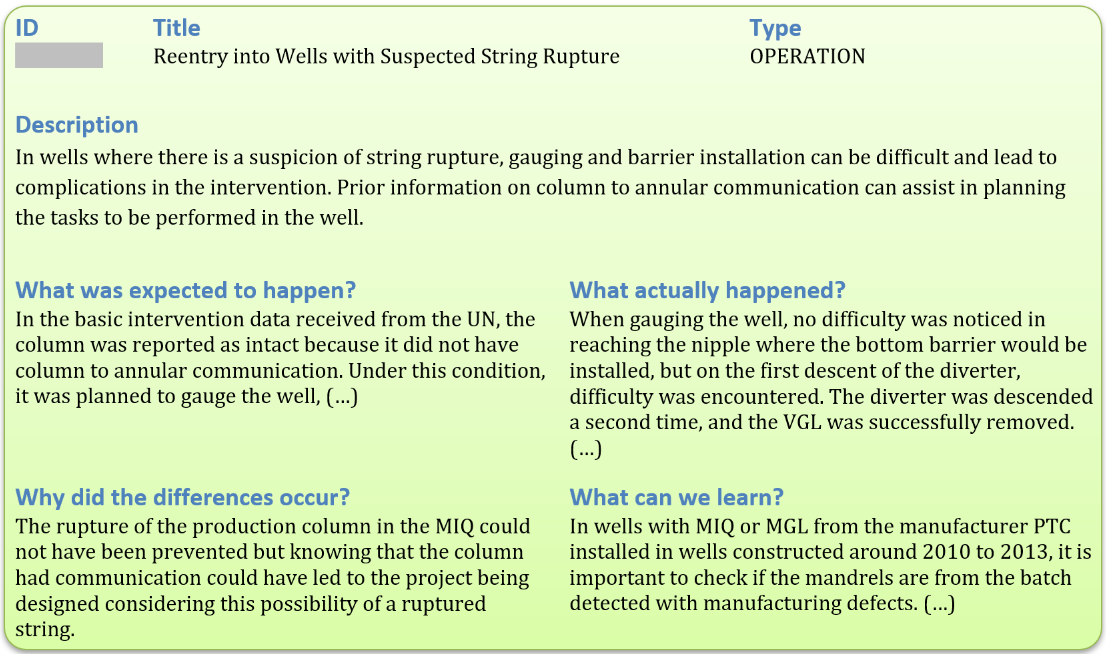
\includegraphics[width=1\textwidth]{images/report_example.png}
  \caption{Amostra de lição aprendida de perfuração e completação. Documento parcial de uma grande empresa de petróleo. (traduzido do português)}
  \label{fig:report_example}
\end{figure}

A implantação de tecnologias de IA enfrenta desafios como dados tendenciosos, alucinações e falta de explicabilidade \cite{Hadi2023}, necessitando de uma abordagem equilibrada. Embora pesquisas anteriores tenham abordado amplamente a IA na indústria, este estudo examina de forma única os desafios e soluções para dados não estruturados complexos em operações de O\&G. Este trabalho aborda a lacuna na compreensão do desempenho de arquiteturas LLM de agente único versus multi-agente em tarefas específicas de domínio, como engenharia de poços, oferecendo insights sobre sua eficácia e relação custo-benefício. A adoção de LLM por uma grande empresa de petróleo destaca o potencial dessas tecnologias para transformar a análise e gestão de dados.

\section{Objetivos}

Esta pesquisa aborda diretamente os desafios enfrentados por grandes empresas de petróleo. Ao investigar as vantagens comparativas e limitações de várias arquiteturas de IA generativa (Gen-AI), incluindo sistemas de agente único e multiagente, este estudo visa identificar as soluções mais eficientes e econômicas.
Os objetivos específicos desta pesquisa são avaliar a adequação e eficácia dos sistemas multiagentes baseados em LLMs para tarefas complexas e específicas de domínios na engenharia de poço, com o objetivo de otimizar o acesso à informação e a tomada de decisões.
O estudo compara sistemas de IA de agente único e multiagente em termos de sua capacidade de responder a consultas relacionadas à engenharia de poços. Ele também mapeia os possíveis obstáculos e limitações associados à implantação de aplicações de Gen-AI.

Os insights obtidos com esta pesquisa visam contribuir diretamente para os objetivos estratégicos das empresas de O\&G, melhorando o acesso a informações sobre engenharia de poços e tarefas de análise de dados automatizadas.
Uma compreensão abrangente dos desafios e limitações associados à Gen-AI permitirá decisões informadas sobre sua adoção, maximizando o retorno sobre o investimento.

\section{Delimitação do Escopo de Negócio}

Para contextualizar o escopo deste estudo, é necessário entender o ciclo de vida de um campo de petróleo, que começa com a Exploração, progride para o Desenvolvimento da Produção, segue com a produção efetiva e culmina no descomissionamento \cite{Badiru2016}. A construção de poços, que envolve a perfuração e completação de poços para extração de hidrocarbonetos, é uma atividade dentro da fase de Desenvolvimento da Produção \cite{Thomas2004}. A Gen-AI tem o potencial de impactar cada uma dessas fases, mas o foco deste trabalho está nas operações das fases de desenvolvimento e manutenção.

A construção de poços é uma atividade altamente especializada que envolve a perfuração e completação de poços para extração de hidrocarbonetos \cite{Thomas2004}. Neste contexto, a Gen-AI pode ser aplicada de várias maneiras. Por exemplo, um chatbot pode gerenciar o conhecimento respondendo a perguntas sobre operações e projetos de poços, recuperando informações dos bancos de dados da organização. Além disso, agentes baseados em LLMs podem ser usados em revisões executivas de projetos para garantir que as operações de perfuração ou completação estejam em conformidade com os padrões da organização e aderem às melhores práticas operacionais. Ademais, a Gen-AI pode realizar inferências em bancos de dados não estruturados para extrair informações específicas de relatórios de texto e obter dados estruturados.

\section{Estrutura da Dissertação}

****SERÁ FEITO POR ÚLTIMO****
